% Chat with PDFs — Multimodal RAG: Architecture, Stack & System Design
% Compile: tectonic architecture.tex  (or pdflatex)
\documentclass[11pt,a4paper]{article}
\usepackage[a4paper,margin=22mm]{geometry}
\usepackage{hyperref}
\usepackage{tikz}
\usetikzlibrary{shapes,arrows,positioning}
\usepackage{booktabs}
\usepackage{enumitem}
\usepackage{xcolor}
\usepackage{graphicx}
\hypersetup{colorlinks=true,linkcolor=blue!60!black,urlcolor=blue!60!black}
\setlength{\parskip}{4pt}
\setlength{\emergencystretch}{2.5em}
\tolerance=2000
\tikzset{
flowbox/.style={rectangle,rounded corners,draw=black,thick,fill=black!4,
  text width=6.2cm,minimum height=1.05cm,align=center,font=\small},
flowstore/.style={ellipse,draw=black,thick,fill=black!8,align=center,font=\small},
flowarr/.style={thick,->,>=stealth}
}
\title{Chat with PDFs: a Multimodal RAG System\\{\large Architecture, Technology Stack \& System Design}}
\author{Project: \texttt{github.com/Divy18s/chat\_with\_pdfs} (2023 $\rightarrow$ 2026 rebuild)}
\date{September 2026}
\begin{document}
\maketitle
\tableofcontents
\newpage

% ============================================================
\section{What was built}
The 2023 prototype was a single-file Streamlit demo
(\texttt{app.py}): PyPDF2 text dump $\rightarrow$ fixed 1000/200 character chunks
$\rightarrow$ in-memory FAISS $\rightarrow$ \texttt{ConversationalRetrievalChain}.
It lost all data on refresh, had no users, no citations, and blocked the UI while indexing.

The 2026 rebuild is a full-stack, multi-user, multimodal RAG product:
{\footnotesize
\begin{center}
\begin{tabular}{@{}lp{4.6cm}p{6.8cm}@{}}
\toprule
Concern & 2023 & 2026 \\
\midrule
Frontend & Streamlit tutorial page & ChatGPT-style 3-pane UI + Next.js 15 scaffold \\
Backend & none (in-process) & Django 6 + Django Ninja (typed, SSE) \\
Database & none & MongoDB (local-JSON fallback) \\
Retrieval & in-memory FAISS & Hybrid RRF: MiniLM + TF-IDF + CLIP \\
Chunking & fixed 1000/200 chars & content-aware: text / table / code / image \\
Vision & none & CLIP vectors + BLIP captions \\
LLM & ChatOpenAI default & Groq \texttt{gpt-oss-120b} (env-switchable) \\
Ingest & blocking button & ThreadPool pages $\times$ files; Celery in Docker \\
Sessions & none & per-chat workspaces, history, delete cascade \\
Deploy & \texttt{streamlit run} & Docker Compose (api, worker, mongo, redis) \\
\bottomrule
\end{tabular}
\end{center}
}

% ============================================================
\section{Technology stack}
{\footnotesize
\begin{center}
\begin{tabular}{@{}lp{4.4cm}p{7.4cm}@{}}
\toprule
Layer & Technology & Role \\
\midrule
UI & Django templates + Tailwind; Next.js 15 + TS (scaffold) & 3-pane chat: history, conversation, per-chat upload \\
API & Django 6, \texttt{django-ninja} 1.7 & typed REST + Server-Sent Events streaming \\
DB & MongoDB 7 (\texttt{pymongo}); local JSON fallback & chats, documents, chunks, messages (audit trail) \\
PDF text & \texttt{pdfplumber} 0.11, \texttt{pypdf} 6, \texttt{PyMuPDF} 1.28 & text + table extraction, image census + rendering \\
Sparse & \texttt{scikit-learn} TF-IDF (1--2 grams) & keyword signal, always available \\
Dense & \texttt{sentence-transformers} 6, MiniLM-L6-v2 384-d; \texttt{torch} 2.14 CPU & semantic signal, \texttt{.npy} per document \\
Vision & CLIP ViT-B/32; BLIP-base (\texttt{transformers} 5) & image vectors + pixels-to-words captions \\
LLM & Groq OpenAI REST (\texttt{urllib}, no SDK) & answers, \texttt{gpt-oss-120b} default \\
Concurrency & \texttt{ThreadPoolExecutor}; Celery + Redis 7 (Docker) & parallel chunking + multi-file ingest \\
Deploy & Docker Compose; Node 20 image & reproducible multi-service stack \\
Docs & \LaTeX\ (Tectonic) + TikZ & this architecture document \\
\bottomrule
\end{tabular}
\end{center}
}

% ============================================================
\section{System architecture}
\subsection{Ingestion pipeline (upload $\rightarrow$ indexed)}
\begin{center}
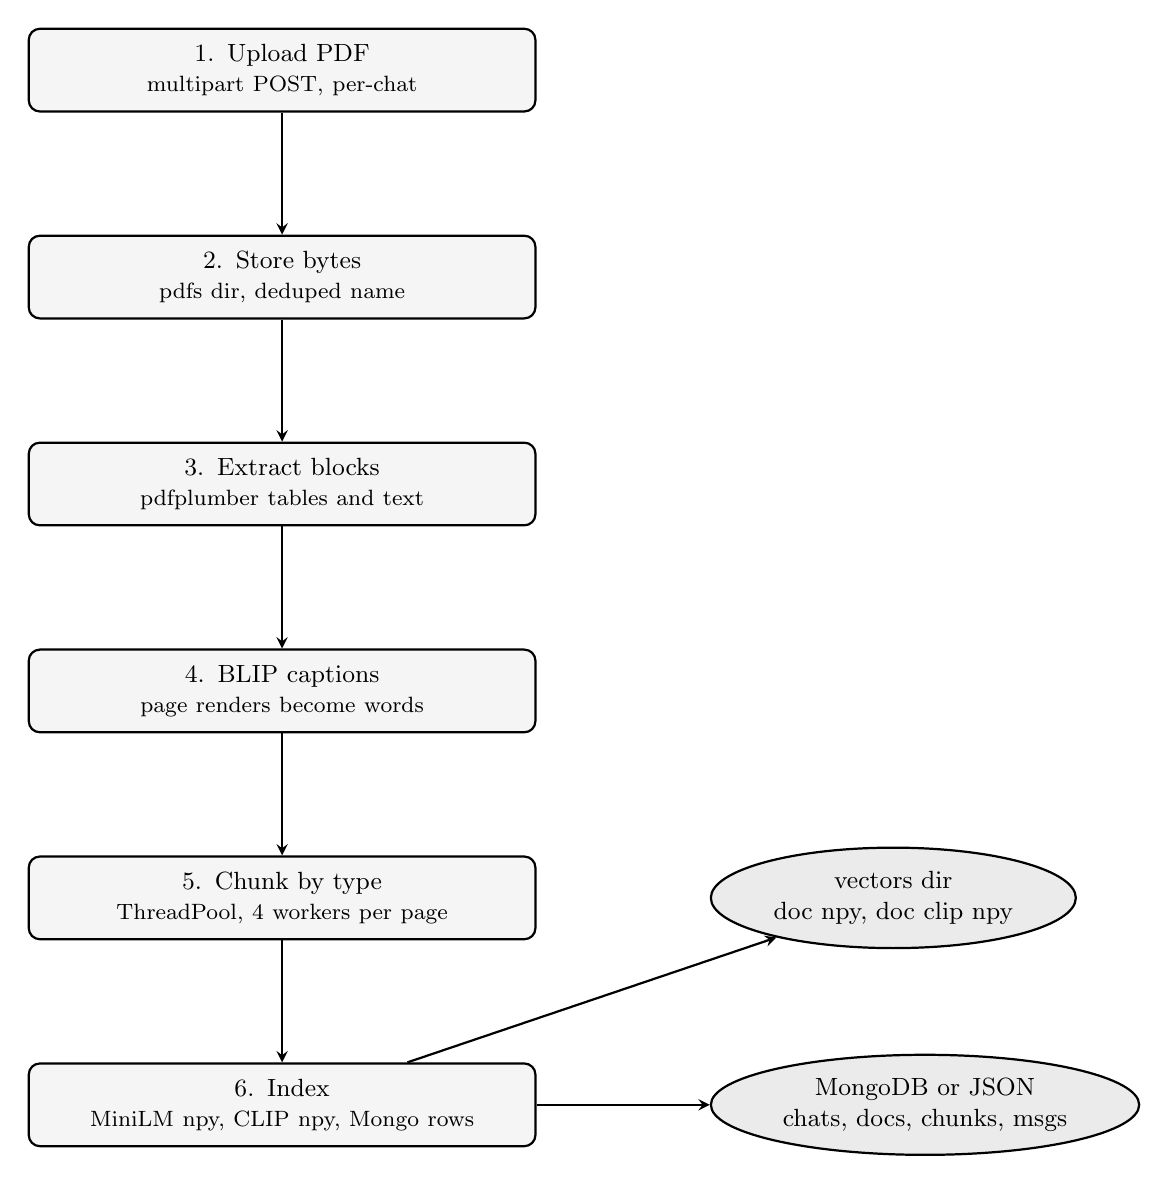
\begin{tikzpicture}[node distance=1.55cm,auto]
\node[flowbox] (up) {1. Upload PDF\\\footnotesize multipart POST, per-chat};
\node[flowbox,below=of up] (store) {2. Store bytes\\\footnotesize pdfs dir, deduped name};
\node[flowbox,below=of store] (ext) {3. Extract blocks\\\footnotesize pdfplumber tables and text};
\node[flowbox,below=of ext] (cap) {4. BLIP captions\\\footnotesize page renders become words};
\node[flowbox,below=of cap] (chk) {5. Chunk by type\\\footnotesize ThreadPool, 4 workers per page};
\node[flowbox,below=of chk] (idx) {6. Index\\\footnotesize MiniLM npy, CLIP npy, Mongo rows};
\node[flowstore,right=2.2cm of idx] (db) {MongoDB or JSON\\chats, docs, chunks, msgs};
\node[flowstore,right=2.2cm of chk] (vec) {vectors dir\\doc npy, doc clip npy};
\draw[flowarr] (up) -- (store);
\draw[flowarr] (store) -- (ext);
\draw[flowarr] (ext) -- (cap);
\draw[flowarr] (cap) -- (chk);
\draw[flowarr] (chk) -- (idx);
\draw[flowarr] (idx) -- (db);
\draw[flowarr] (idx) -- (vec);
\end{tikzpicture}
\end{center}

\subsection{Query pipeline (question $\rightarrow$ streamed answer)}
\begin{center}
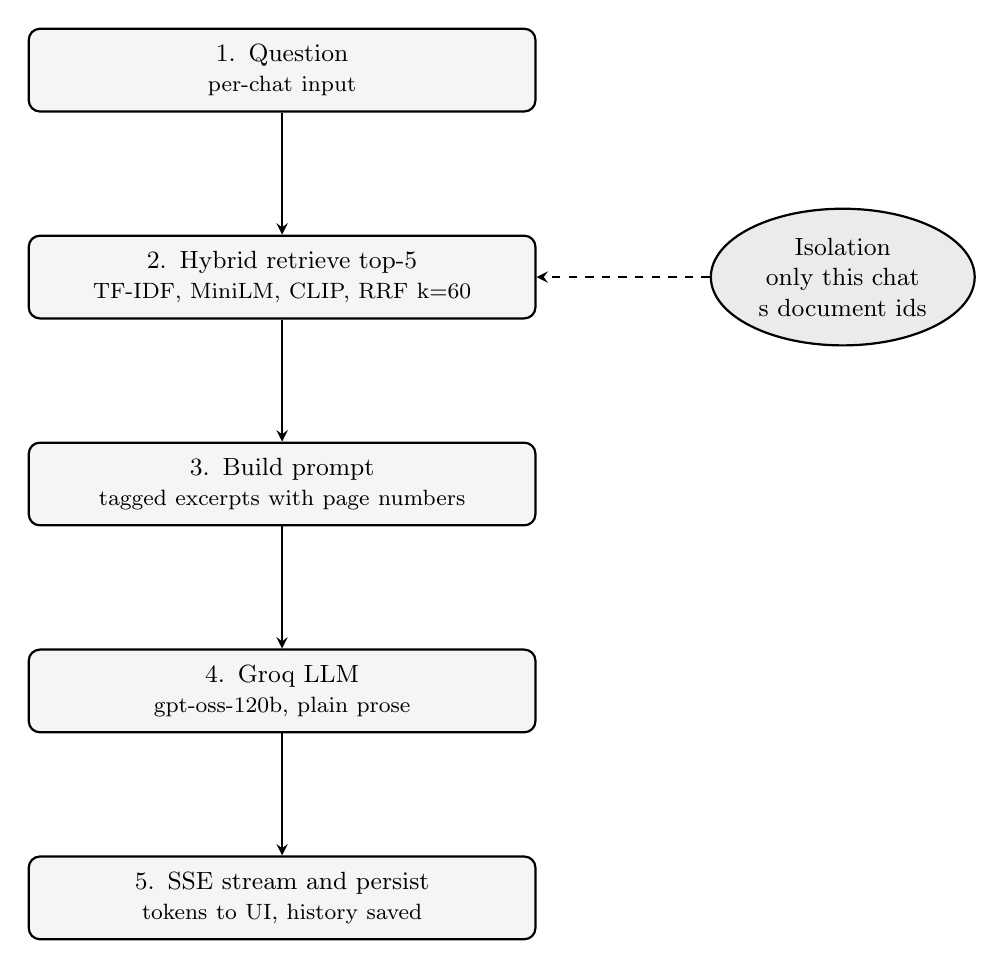
\begin{tikzpicture}[node distance=1.55cm,auto]
\node[flowbox] (q) {1. Question\\\footnotesize per-chat input};
\node[flowbox,below=of q] (r) {2. Hybrid retrieve top-5\\\footnotesize TF-IDF, MiniLM, CLIP, RRF k=60};
\node[flowbox,below=of r] (p) {3. Build prompt\\\footnotesize tagged excerpts with page numbers};
\node[flowbox,below=of p] (l) {4. Groq LLM\\\footnotesize gpt-oss-120b, plain prose};
\node[flowbox,below=of l] (s) {5. SSE stream and persist\\\footnotesize tokens to UI, history saved};
\node[flowstore,right=2.2cm of r] (scope) {Isolation\\only this chat\\s document ids};
\draw[flowarr] (q) -- (r);
\draw[flowarr] (r) -- (p);
\draw[flowarr] (p) -- (l);
\draw[flowarr] (l) -- (s);
\draw[flowarr,dashed] (scope) -- (r);
\end{tikzpicture}
\end{center}

\subsection{Deployment (Docker Compose)}
API and worker share one image with different commands (stateless, horizontally scalable).
State lives in volumes: \texttt{mongo\_data} (documents/chunks/history), vector files, PDF dir.
\texttt{frontend:3000} $\rightarrow$ \texttt{api:8000} $\rightarrow$ \texttt{mongo:27017, redis:6379};
\texttt{docker compose up --scale worker=3} demonstrates ingestion scaling.

% ============================================================
\section{Step-by-step: technology, function, handling}
\subsection{Step 1 -- Upload and chat sessions}
\textbf{Tech:} Django Ninja \texttt{File} upload; \texttt{chats} collection (\texttt{db.py}).\\
\textbf{Does:} creates one workspace per chat holding its own \texttt{doc\_ids}; filenames deduped on disk.\\
\textbf{Handles:} non-PDF rejected (400); unknown chat id $\rightarrow$ 404; multi-file endpoint fans out on threads and reports per-file errors plus \texttt{total\_ms}.

\subsection{Step 2 -- Extraction (text, tables, images)}
\textbf{Tech:} \texttt{pdfplumber} primary, threaded \texttt{pypdf} fallback,
\texttt{PyMuPDF} census (\texttt{extract\_blocks}).\\
\textbf{Does:} emits typed blocks \texttt{\{kind: text$|$table$|$image, page, text\}}; tables serialized to GitHub-flavour markdown.\\
\textbf{Handles:} borderless tables fall back to text (still page-cited); missing \texttt{pdfplumber} $\rightarrow$ pypdf path; corrupt PDF $\rightarrow$ clean 400, nothing half-indexed.

\subsection{Step 3 -- Vision enrichment (pixels to words)}
\textbf{Tech:} PyMuPDF 72\,dpi page renders; BLIP-base captioning; page-text excerpts.\\
Code: \texttt{extract\_page\_images}, \texttt{caption\_images}.
\textbf{Does:} each image block gains \texttt{Visual: $<$caption$>$} plus up to 400 chars of neighbouring page text.\\
\textbf{Handles:} no-image pages skipped; BLIP failure $\rightarrow$ caption omitted, CLIP + proxy still work (\texttt{USE\_CAPTION=0} disables).

\subsection{Step 4 -- Content-aware chunking}
\textbf{Tech:} recursive splitter + heading prefix; whole-table rule; code line rule (\texttt{chunk\_block}).\\
\textbf{Does:} text 800/120 chars keeping sentence/paragraph boundaries; tables exactly one chunk (never split mid-row); code 600/80 preserving lines; images one chunk.\\
\textbf{Handles:} code detected by indentation/keywords; borderless tabular text caught by column heuristic; tiny fragments ($<$20 chars) dropped.

\subsection{Step 5 -- Dense and vision indexing}
\textbf{Tech:} MiniLM-L6-v2 (384-d, normalized) and CLIP ViT-B/32 (512-d), NumPy row stores (\texttt{embeddings.py}).\\
\textbf{Does:} writes \texttt{vectors/\{doc\}.npy} aligned to chunk idx and \texttt{\{doc\}.clip.npy} aligned to image chunks; upload response reports \texttt{dense/dim/vision}.\\
\textbf{Handles:} encoder/model failure $\rightarrow$ sparse-only mode; old docs without \texttt{.npy} encoded on the fly once; \texttt{USE\_DENSE=0}/\texttt{USE\_VISION=0} force fallbacks.

\subsection{Step 6 -- Hybrid retrieval with RRF}
\textbf{Tech:} TF-IDF cosine + MiniLM cosine + CLIP cosine fused by Reciprocal Rank Fusion, k=60 (\texttt{hybrid\_order}); optional CrossEncoder rerank.\\
\textbf{Does:} three rank lists vote; visual-intent queries (colour/figure/chart/show words) with confident CLIP ($>$0.20) pin image hits first; text queries unaffected.\\
\textbf{Handles:} verified -- ``red square'' returns the image chunk first, ``capital of France'' the text chunk; any signal can fail closed while the rest answer.

\subsection{Step 7 -- Prompt and generation}
\textbf{Tech:} Groq OpenAI-compatible REST via \texttt{urllib} (no SDK pin risk); model from env (\texttt{groq\_client.py}).\\
\textbf{Does:} top-5 excerpts tagged \texttt{[TABLE]/[TEXT]/[CODE]/[IMAGE]} with page numbers; system prompt demands plain ChatGPT-style prose, no citation markers.\\
\textbf{Handles:} missing key $\rightarrow$ explicit error; Groq-side decommissioned models surfaced with 400 text (Qwen was retired mid-project; default moved to \texttt{gpt-oss-120b}).

\subsection{Step 8 -- Streaming and persistence}
\textbf{Tech:} \texttt{StreamingHttpResponse} SSE stream; history saved
\emph{before} streaming (\texttt{chat\_stream\_s}).\\
\textbf{Does:} word tokens stream into the bubble; on \texttt{[DONE]} the UI reloads persisted history -- nothing vanishes; SSE errors show a hint instead of silent loss.\\
\textbf{Handles:} server restart mid-stream $\rightarrow$ \texttt{onerror} message pointing at \texttt{/api/health}.

\subsection{Step 9 -- Deletion cascade}
\textbf{Tech:} \texttt{DELETE /api/chats/id} $\rightarrow$ \texttt{db.delete\_chat}
(+ embedding cleanup).\\
\textbf{Does:} removes chat, documents, chunks, messages, PDF bytes, MiniLM and CLIP vectors. Verified: other chats untouched.\\
\textbf{Handles:} asks confirmation in UI; Mongo and JSON-fallback paths both covered.

% ============================================================
\section{System design decisions (interview-ready)}
\begin{enumerate}[leftmargin=1.2cm]
\item \textbf{Stateless API + stateful stores.} Django/Celery containers hold no state; MongoDB, vector files, PDFs live in volumes. Scale workers without data loss.
\item \textbf{Tenant isolation per chat.} Every retrieval filters by \texttt{chat.doc\_ids} (proven: finance chat cannot see Paris notes). Same pattern as SaaS tenant scoping.
\item \textbf{Async-friendly ingest.} ThreadPool today (pages $\times$ files, \texttt{total\_ms} reported), Celery+Redis in Docker for true background jobs with retries.
\item \textbf{Graceful degradation ladder:} vision $\rightarrow$ dense $\rightarrow$ sparse. A missing GPU/model never pages the user.
\item \textbf{Audit trail.} All Q/A pairs persisted per chat -- replayable, evaluable, demoable.
\item \textbf{Three-signal retrieval over one index.} Avoids operating Qdrant locally while keeping the RRF story; Qdrant HNSW is the named production swap.
\item \textbf{Secrets hygiene.} Bare-\texttt{gsk\_} \texttt{.env} accepted locally; \texttt{.env.example} documents Docker format; keys never baked into images.
\end{enumerate}

% ============================================================
\section{Research foundations}
{\footnotesize
\begin{center}
\begin{tabular}{@{}lp{9.0cm}@{}}
\toprule
Paper / method & What we took from it \\
\midrule
RAG, Lewis et al.\ 2020 & retrieve-then-generate baseline architecture \\
Self-RAG, Asai et al.\ 2023 & self-grading + retry loop (documented stretch) \\
Corrective RAG, Yan et al.\ 2024 & rewrite/retry on weak evidence (stretch) \\
HyDE, Gao et al.\ 2022 & hypothetical-answer retrieval for vague queries (stretch) \\
Lost in the Middle, Liu et al.\ 2023 & justification for reranking top hits \\
Late Chunking, J.\,G\"unther et al.\ (Jina AI) 2024 & embed-then-chunk analysed; deferred (needs long-context encoder) \\
RAPTOR 2024 & hierarchical summaries (deferred) \\
RRF, Cormack et al.\ 2009 & k=60 fusion of our three rank lists \\
CLIP, Radford et al.\ 2021 & shared text--image space for visual retrieval \\
BLIP, Li et al.\ 2022 & bootstrapped captioning for pixels-to-words \\
ColPali/ColQwen, Faysse et al.\ 2024 & page-level vision embeddings (deferred, scan-only use case) \\
\bottomrule
\end{tabular}
\end{center}
}

% ============================================================
\section{Verification performed}
\texttt{manage.py check} clean; upload/index/chat/delete exercised via Django test client:
health \texttt{\{dense:true, dim:384, vision:true\}}; grid-table PDF $\rightarrow$ \texttt{\{text:1, table:1\}};
``Q1 revenue?'' answered with both text+table hits; ``red square'' $\rightarrow$ image chunk first;
``capital of France'' $\rightarrow$ text first; chat delete removed PDF + both \texttt{.npy} files
leaving other chats intact; SSE persistence bug reproduced and fixed (save-before-stream).

% ============================================================
\section{Thirty-second pitch}
``ChatGPT for PDFs, rebuilt as a real system: per-chat workspaces with isolated documents,
a threaded multimodal ingest that treats text, tables, code and figures differently,
and a three-signal hybrid retriever -- MiniLM dense plus TF-IDF sparse plus CLIP vision
fused with RRF -- with BLIP captions so the LLM can describe images. Stateless Django API,
MongoDB audit trail, SSE streaming, Docker Compose for scale-out.''

\appendix
\section{API reference}
\texttt{GET /api/health}, \texttt{GET/POST /api/chats}, \texttt{GET/DELETE /api/chats/\{id\}},
\texttt{POST /api/chats/\{id\}/upload}, \texttt{GET .../documents}, \texttt{GET .../messages},
\texttt{POST .../chat}, \texttt{GET .../stream?q=}; legacy global \texttt{/api/documents},
\texttt{/api/chat}, \texttt{/api/chat/stream}, \texttt{POST /api/documents/upload-many}.
Flags: \texttt{GROQ\_MODEL}, \texttt{EMBED\_MODEL}, \texttt{USE\_DENSE}, \texttt{USE\_VISION},
\texttt{USE\_CAPTION}, \texttt{USE\_RERANK}, \texttt{MONGO\_URI}, \texttt{RAG\_TOP\_K}.
\end{document}
